\section{Scaling Hypothesis Part II and Renormalization Group}
\subsection{Recap}
We postulate a free energy:
\begin{equation}
    f_{\text{sing}}(t, h) = \abs{t}^{2-\alpha}g(h/\abs{t}^\Delta)
\end{equation}
where the exponents are different from those appearing in mean field theory, and $g$ is a homogenous function of its argument. From this, we are able to derive for a scaling law for the magnetization $m$, for the specific heat $C$, the susceptibility $\chi$, etc.

If this holds, we have a correlation length:
\begin{equation}
    \xi(t, h) = \abs{t}^{-\nu}g_\xi(h/\abs{t}^\Delta).
\end{equation}
In MF theory, $\nu = 1/2$, but it may be different here. We will find $\mu > 0$ so the correlation length diverges as $T \to T_c$.

We assume that $\ln Z$ is extensive, i.e. $\propto L^d$ (it is very rare that this would not be the case). More specifically, $\ln Z \propto \frac{L^d}{\xi^d}$ plus any nonsingular terms. Then the free energy goes as:
\begin{equation}\label{eq:singfreeenergy}
    f_{\text{sing}} = \frac{\ln Z}{L^d}g(h/\abs{t}^\Delta) \propto \abs{t}^{d\nu}g(\cdot)
\end{equation}
which implies:
\begin{equation}
    2-\alpha = d\nu
\end{equation}
This is known as the hyperscaling, or Josephson relation. It doesn't work in MF theory, unless $d = 4$. In one of the homework problems, we will muse on why this is.

We study the correlation function:
\begin{equation}
    G(\gamma, 0) = \avg{m(\gamma)m(0)} - \avg{m}^2 \sim \frac{1}{\abs{\gamma}^{d-2+\eta}}
\end{equation}

\begin{figure}[htbp]
    \centering
    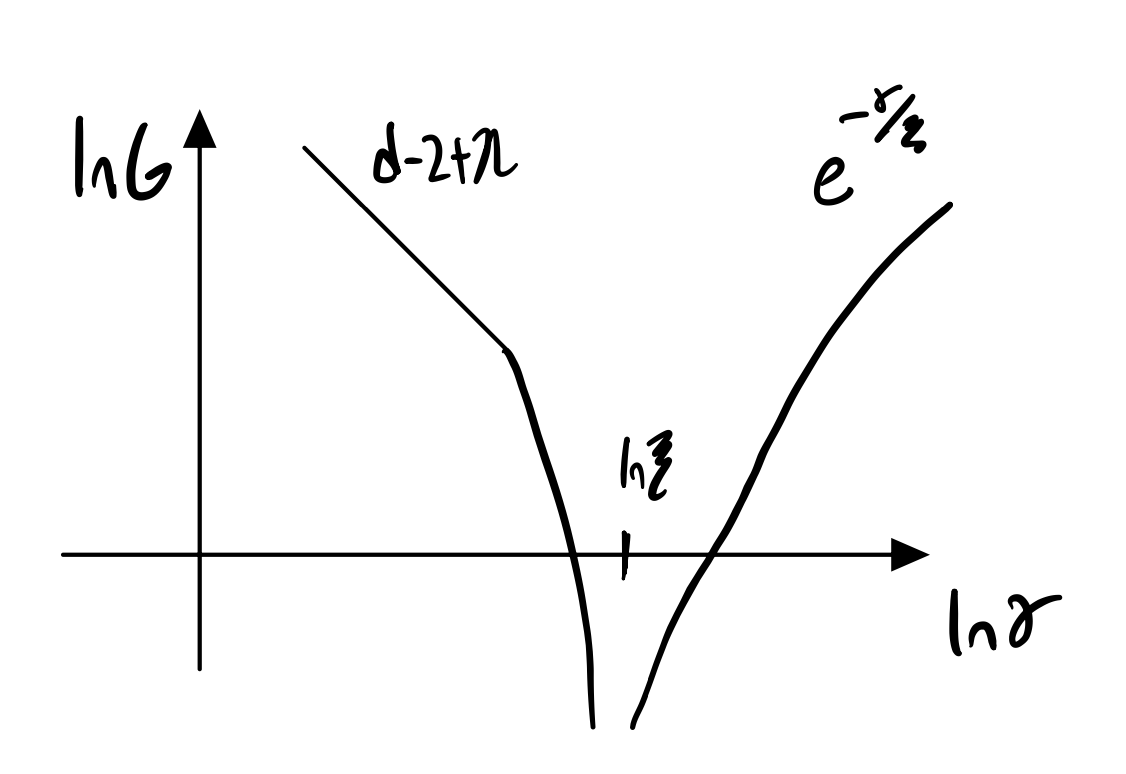
\includegraphics[scale=0.5]{Lectures/Figures/correlation_scaling.png}
    \caption{At long distances, the correlation functions die off exponentially. Near the critical point, it is a power law.}
    \label{fig:correlation_scaling}
\end{figure}

We now study the renormalization group, which allows us to mathematically obtain these exponents. We start with a conceptual view.

\subsection{Renormalization Group: Conceptual View}
\subsubsection*{Step 1: Coarse Graining}
We do RG via a process of coarse graining. We take a length scale $x$, and convert it to $bx$ where $b > 1$. Pictorially, we look at a $bx \times bx$ block of spins and average them to form an ``averaged spin'' corresponding to that whole block. I.e. the magnetization as a function of $x$ becomes:
\begin{equation}
    m(x) = \frac{1}{b^d}\int d^dx' m(x')
\end{equation}
where we integrate over the cell center at $x$.

\begin{figure}[htbp]
    \centering
    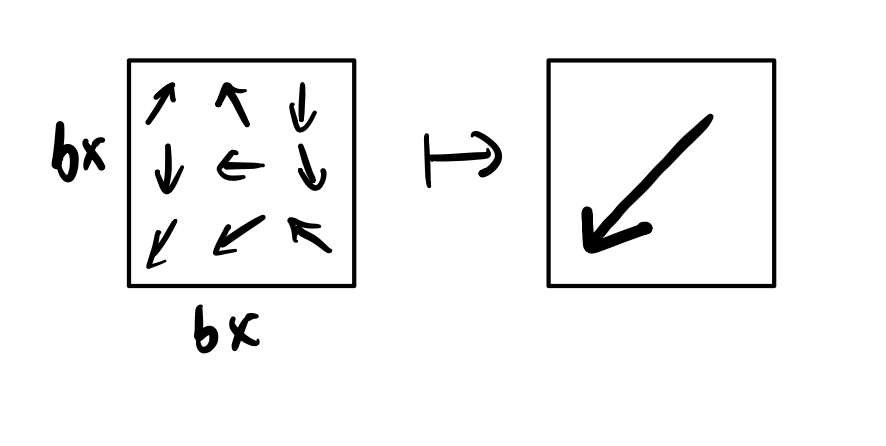
\includegraphics[scale=0.5]{Lectures/Figures/blockspins.png}
    \caption{At the coarse graining step, we integrate over a block of spins and replace it with the average.}
    \label{fig:blockspins}
\end{figure}

Notice that we lose information when we do this. Via course graining, we lose the microscopics.

\subsubsection*{Step 2: Rescale}
We now take $x_{\text{new}} = \frac{x_{\text{old}}}{b}$, rescaling/blowing up the new cell size to be the size of the original unit cell.

\subsubsection*{Step 3: Renormalize}
We renormalize the magnetization:
\begin{equation}
    m_{\text{new}}(x_{\text{new}}) = \frac{1}{\xi b^d}\int d^dx'm(x')
\end{equation}
Where to make the theory look the same as when we started, we introduce a new renormalization parameter $\xi$.

\subsection{Getting Exponents out of RG}

Having done this, we can construct a new probability distribution:
\begin{equation}
    W[m_{\text{new}}] = e^{-\beta H_b[m_{\text{new}}]}
\end{equation}

We will assert that at criticality ($t = h = 0$), the Hamiltonian is statistically similar to the one I had originally. This means of course that in this theory, we introduce a new effective temperature and field that must be a function of the old ones. I.e.:
\begin{equation}
    \begin{split}
        t_{\text{new}} &= f(t_{\text{old}}, h_{\text{old}})
        \\ h_{\text{new}} &= f'(t_{\text{old}}, h_{\text{old}})
    \end{split}
\end{equation}
but we have some constraints. $(0, 0) \to (0, 0)$, and $t_{\text{new}}, h_{\text{new}}$ should grow. Since we rescale the length, the correlation length should get shorter, so we grow away from the $0$ point. We also hope that there is no singular behaviour in these functions. Finally, we want to preserve the symmetry; as such, we will not mix $t$ with $h$. Then:
\begin{equation}
    \begin{split}
        t_b(t, h) &= A(b)t + O(t^2)
        \\ h_b(t, h) &= B(b)h + O(h^2)
    \end{split}
\end{equation}
We know that:
\begin{equation}
    A(1) = B(1) = 1
\end{equation}
(This corresponds to no scaling). There is also the assumption that this could be repeated:
\begin{equation}
    t_{b_1b_2}(t, h) = A(b_1b_2)t = A(b_1)A(b_2)t
\end{equation}
In other words, scaling once by $b_1b_2$ should be the same as scaling by $b_2$ and then $b_1$. This implies that:
\begin{equation}
    A(b) \sim b^{y_t} \quad B(b) \sim b^{y_h}
\end{equation}
Notice that this is a semigroup, as we can only go one way. So, this isn't actually a group (Renormalization group is a bit of a misnomer). This is how we can see the ``loss in information'' of this process.

We also assume that $y_t, y_h > 0$. So, we go further from the critical point. This might cause us concern because then the higher order $t^2, h^2$ terms in the scaling may become relevant. But indeed we take $b \sim 1$ in order to stay within a neighbourhood of the critical point, as this is the only regime in which this analysis is actually valid. Then, looking at the the scaling of the general functions:
\begin{equation}
    X(t, h) = b^{y_x}X(b^{y_t}t, b^{y_h}h)
\end{equation}
and the new configuration becomes:
\begin{equation}
    Z = \int \mathcal{D}mW[m]
\end{equation}
but the weights of the old configuration should be the same as the old one, so:
\begin{equation}
    Z = \int \mathcal{D}mW[m] = \int \mathcal{D}m' W[m'] = Z'
\end{equation}
Which then leads us to conclude that:
\begin{equation}
    Vf(t, h) = V'f(t',h')
\end{equation}
So then looking at the scaling of the free energy:
\begin{equation}
    f(t, h) \sim \frac{1}{b^d}f(b^{y_t}t, b^{y_h}h)
\end{equation}
We now have to propose a trajectory to scale such that we eventually get to the form $\abs{t}^{2-\alpha}g(h/\abs{t}^\Delta)$. We take $b^{y_t}t \sim 1$ so $b\sim t^{-1/y_t}$. Then:
\begin{equation}
    f(t, h) = \frac{1}{b^d}f(1, h/t^{y_h/y_t})
\end{equation}
So, we are taking the free energy, positing a scaling form, and we get out something that looks like Eq. \eqref{eq:singfreeenergy} as we desired.

From this, we obtain:
\begin{equation}
    2 - \alpha = \frac{d}{y_t}
\end{equation}
\begin{equation}
    \Delta = \frac{y_h}{y_t}
\end{equation}
What we will do is find a scaling path and determine the scaling exponents $y_h, y_t$, and then this tells us about the critical exponents of our interest. Let's look at the others.

There will now be a new correlation length:
\begin{equation}
    \chi' = \chi/b
\end{equation}
Looking at the general form of the scaling of the correlation length:
\begin{equation}
    \chi(t, h)= b\chi(b^{y_t}t, b^{y_h}h) = t^{-1/y_t}\xi(1, h/t^{y_h/y_t}) 
\end{equation}
and thus:
\begin{equation}
    \nu = -\frac{1}{y_t} = \frac{2-\alpha}{d}
\end{equation}
which is the Josephson scaling relation.

Let us look at the magnetization as well"
\begin{equation}
    m(t, h) = \frac{1}{V}\dpd{\ln Z}{h} = b^{y_h - d}m(1, h/t^{y_h/y_t})
\end{equation}
so then:
\begin{equation}
    \beta = \frac{d}{y_t} - \frac{y_h}{y_t} = 2-\alpha-\Delta
\end{equation}

\subsection{RG Fixed Points and Flows}
To start, we write down the most general Hamiltonian allowed by symmetry. For example here:
\begin{equation}
    \beta H = \int d^d x\left[\frac{1}{2}tm^2 + \frac{1}{4}um^4 + \frac{1}{6}vm^6 + \frac{1}{2}K(\nabla m)^2 + \frac{1}{2}L(\nabla^2 m)^2 + \ldots\right]
\end{equation}
I now have a parameter space $S(t, u,  v, K, L, \ldots)$ in which the parameters define a point.

Then, we'll go through the RG process. We course grain by averaging over block size $b$, rescale $x \to x/b$, then normalize by $\xi$. We then have the magnetization:
\begin{equation}
    m'(x') = \frac{1}{\xi b^d}\int d^dxm(x)
\end{equation}
We then construct $P[m']$ from $P[m]$ (nontrivial process!). We then get a rescaled Hamiltonian $H'(t', u', v', K', L', \ldots)$. This process is the same as saying that:
\begin{equation}
    S' = R_b S
\end{equation}
i.e. we have applied a map to our parameter space.

We consider a deviation:
\begin{equation}
    S^*_\alpha + \delta S_\alpha' = S_\alpha^* + (R_b)_{\alpha\beta}\delta S'_\beta
\end{equation}
where $S^*$ is the fixed point of the RG theory (imagine we have done the calculation and found this point/the critical point), i.e.:
\begin{equation}
    R_bS^* = S^*
\end{equation}
and $\xi(S^*) = b\xi(R_b S^*)$ i.e. $\xi \to \infty$. We can write the renormalization group map (the $L$ denoting the linearized version of the map, which we assume we can do in the vicinity of the critical point) as:
\begin{equation}
   (R^L_b)_{\alpha\beta} = \dpd{S'_\alpha}{S_\beta}
\end{equation}
i.e. the RG takes us from $S_\alpha$ to $S'_\alpha$. Now, consider this map to have eigenvectors $\Theta_i$ and eigenvalues $\lambda(b)_i$. Then:
\begin{equation}
    R_b^L R_{b'}^L\Theta_i = \lambda_i(n)\lambda_i(b') = \lambda_i(b'b').
\end{equation}
thus:
\begin{equation}
    \lambda_i(b) \sim b^{y_i}
\end{equation}
Therein, the $\Theta_i$ correspond to scaling directions and the $y_i$ correspond to anomalous dimensions (in MF theory they are all 1 - not anomalous). We now expand $S$ around the fixed point based on these scaling directions:
\begin{equation}
    S = S^* + \sum_i g_i \Theta_i
\end{equation}
After we scale:
\begin{equation}
    S' = S^* + \sum_i g_i b^{y_i}[\Theta]
\end{equation}
Pictorally, we have the flows in Fig. \ref{fig:RGflows}.

\begin{figure}[htbp]
    \centering
    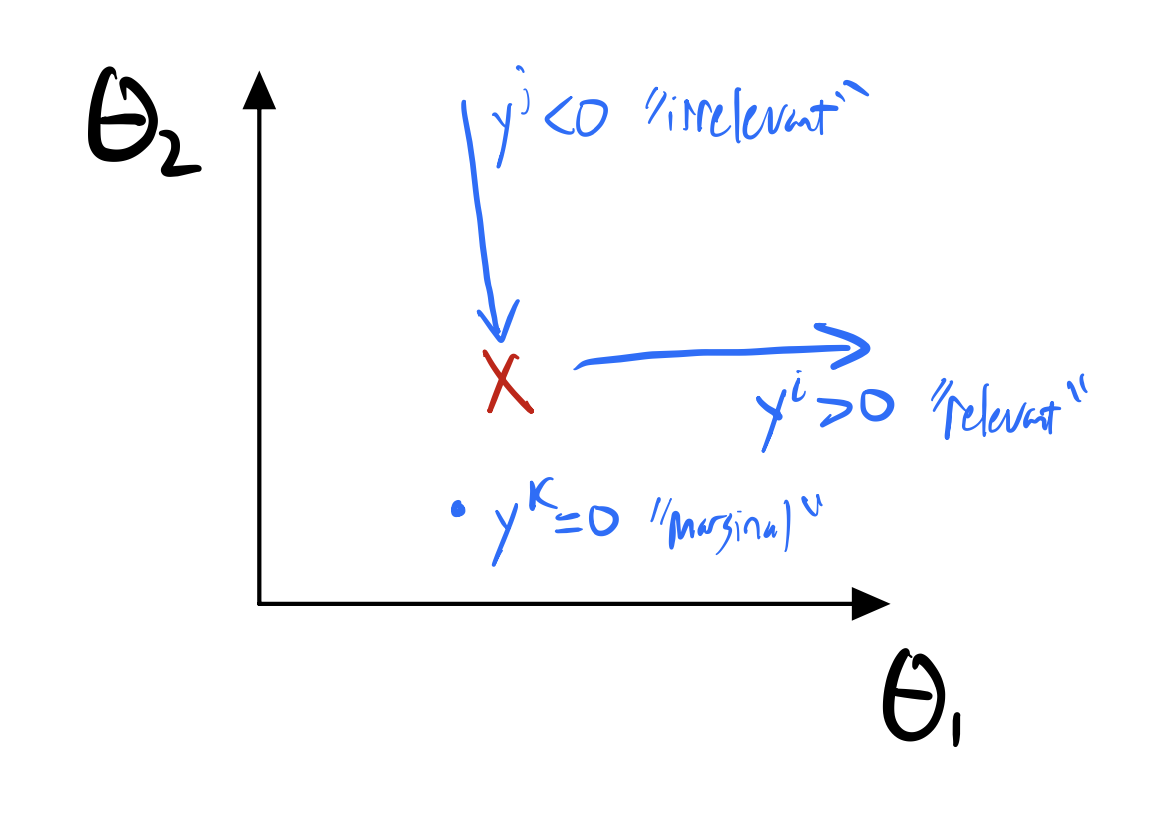
\includegraphics[scale=0.5]{Lectures/Figures/RGflows.png}
    \caption{Different eigenvectors have different flow properties. Irrelevant eigenvectors go towards the fixed point, relevant eigenvectors flow away, and marginal eigenvectors are stationary.}
    \label{fig:RGflows}
\end{figure}

The vectors define a basin of attraction. Relevant means the eigenvectors go away from the fixed point, so the fluctuations grow and become important. Irrelevant mean the eigenvectors go towards the fixed point, so the fluctuations vanish (hence irrelevant). Finally, we have $y_i = 0$ and then we call the flows ``marginal''. These directions correspond to some linear combinations to linear combinations of the parameters $t, u, v, K, L,\ldots$ of the theory. The main takeaway is that this flow analysis tells us what variables are the important ones.

Next Wednesday, we will go through this process for the Gaussian theory, and identify the Wilson-Fisher fixed point.